\chapter{Análise Estatística das Questões do Questionário}\label{ape:analise-estatistica-questionario}

\textbf{Questão 1: Os itens recomendados corresponderam com os meus interesses.}

\begin{figure}[htb]
  \caption{\label{fig:questao1-boxplot}Boxplot da questão 1}
  \begin{center}
      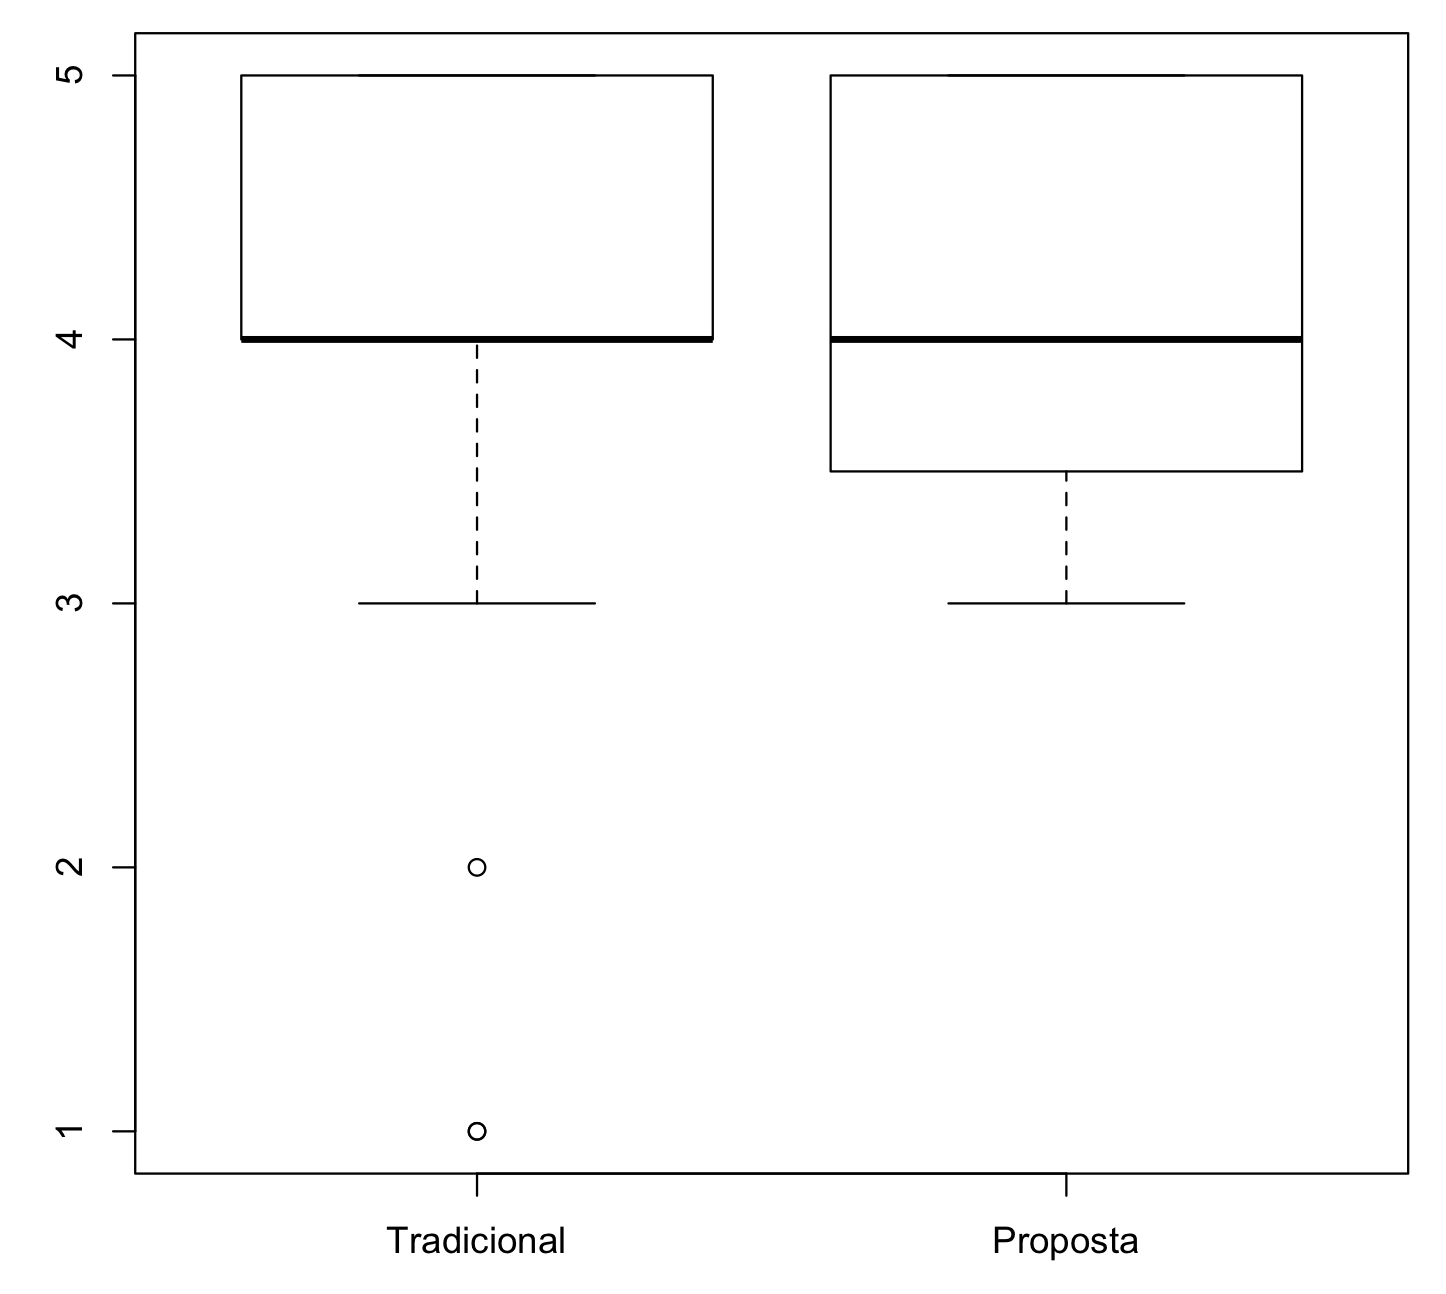
\includegraphics[scale=0.4]{./Figuras/questao1-boxplot.png}
  \end{center}
  \legend{Fonte: O autor.}
\end{figure}

\begin{multicols}{2}

\noindent\textbf{Tradicional}\\
Min.   :1.000\\
1st Qu.:4.000\\
Median :4.000\\
Mean   :4.032\\
3rd Qu.:5.000\\
Max.   :5.000\\
\columnbreak

\noindent\textbf{Proposta}\\
Min.   :3.000\\
1st Qu.:3.750\\
Median :4.000\\
Mean   :4.042\\
3rd Qu.:5.000\\
Max.   :5.000
\end{multicols}

Wilcoxon rank sum test with continuity correction

\noindent
data:  $data\_1\_tradicional$ and $data\_1\_proposta$\\
W = 404, p-value = 0.5635\\
alternative hypothesis: true location shift is not equal to 0

\textbf{Resultado: Aceita a hipótese nula - Sem diferença significativa}

\newpage
\textbf{Questão 2: Os itens recomendados para mim são diversificados (o sistema se preocupa em trazer itens diferentes a cada recomendação).}

\begin{figure}[htb]
  \caption{\label{fig:questao2-boxplot}Boxplot da questão 2}
  \begin{center}
      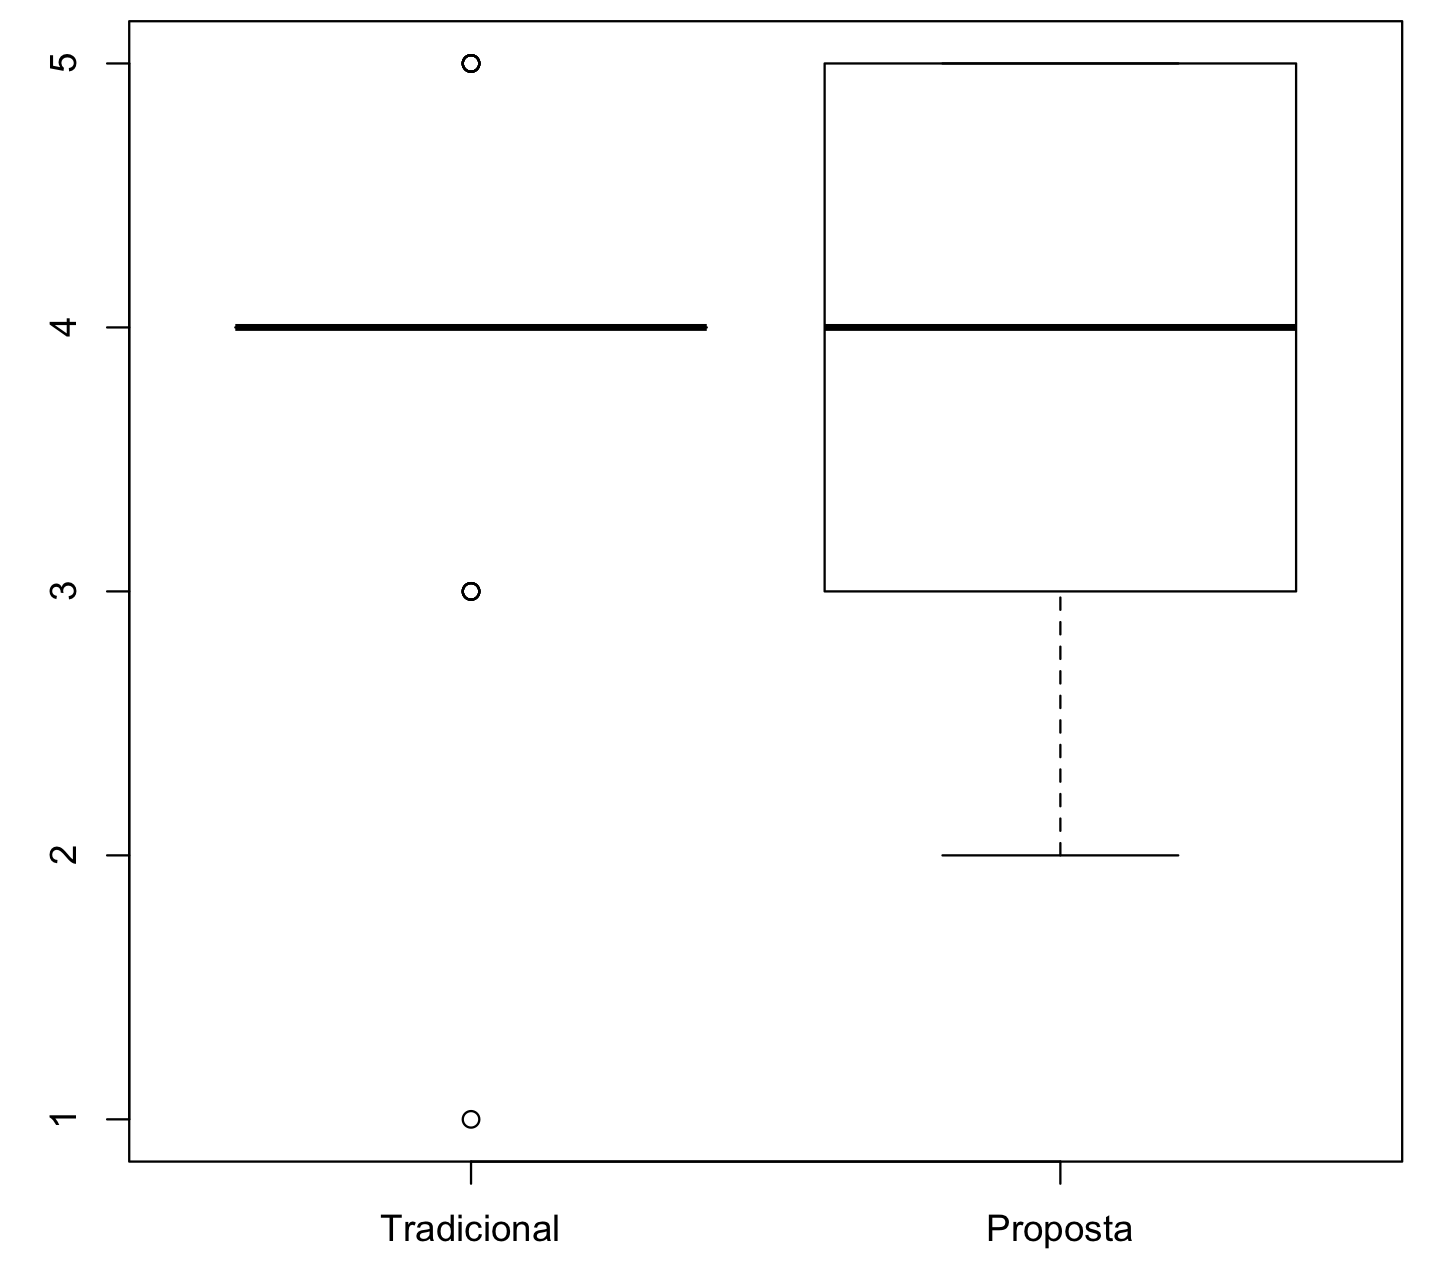
\includegraphics[scale=0.4]{./Figuras/questao2-boxplot.png}
  \end{center}
  \legend{Fonte: O autor.}
\end{figure}

\begin{multicols}{2}

\noindent\textbf{Tradicional}\\
Min.   :1.000\\
1st Qu.:4.000\\
Median :4.000\\
Mean   :3.933\\
3rd Qu.:4.000\\
Max.   :5.000\\
\columnbreak

\noindent\textbf{Proposta}\\
Min.   :2\\
1st Qu.:3\\
Median :4\\
Mean   :4\\
3rd Qu.:5\\
Max.   :5
\end{multicols}

Wilcoxon rank sum test with continuity correction

\noindent
data:  $data\_2\_tradicional$ and $data\_2\_proposta$\\
W = 376.5, p-value = 0.8178\\
alternative hypothesis: true location shift is not equal to 0

\textbf{Resultado: Aceita a hipótese nula - Sem diferença significativa}

\newpage
\textbf{Questão 3: Os itens recomendados corresponderam aos  interesses e necessidades que eu tinha no momento.}

\begin{figure}[htb]
  \caption{\label{fig:questao3-boxplot}Boxplot da questão 3}
  \begin{center}
      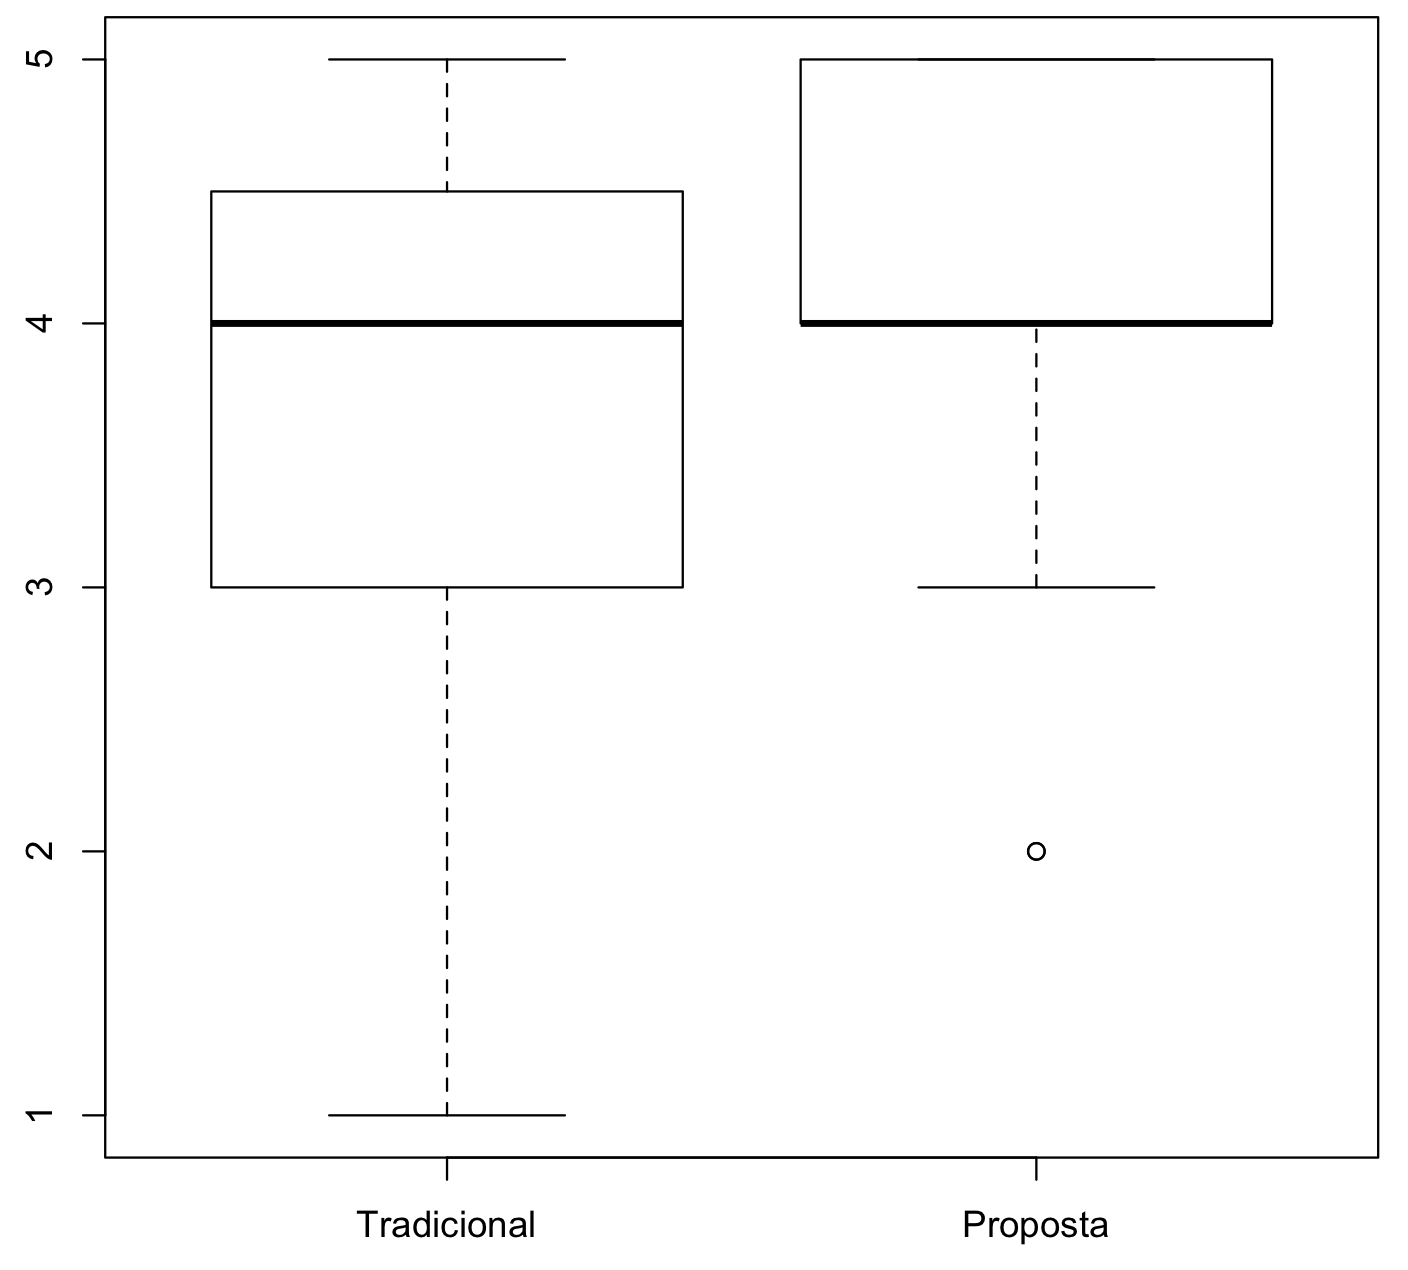
\includegraphics[scale=0.4]{./Figuras/questao3-boxplot.png}
  \end{center}
  \legend{Fonte: O autor.}
\end{figure}

\begin{multicols}{2}

\noindent\textbf{Tradicional}\\
Min.   :1.000\\
1st Qu.:3.000\\
Median :4.000\\
Mean   :3.806\\
3rd Qu.:4.500\\
Max.   :5.000\\
\columnbreak

\noindent\textbf{Proposta}\\
Min.   :2\\
1st Qu.:4\\
Median :4\\
Mean   :4\\
3rd Qu.:5\\
Max.   :5
\end{multicols}

Wilcoxon rank sum test with continuity correction

\noindent
data:  $data\_3\_tradicional$ and $data\_3\_proposta$\\
W = 364, p-value = 0.5119\\
alternative hypothesis: true location shift is not equal to 0

\textbf{Resultado: Aceita a hipótese nula - Sem diferença significativa}

\newpage
\textbf{Questão 4: As recomendações são feitas no momento adequado.}

\begin{figure}[htb]
  \caption{\label{fig:questao4-boxplot}Boxplot da questão 4}
  \begin{center}
      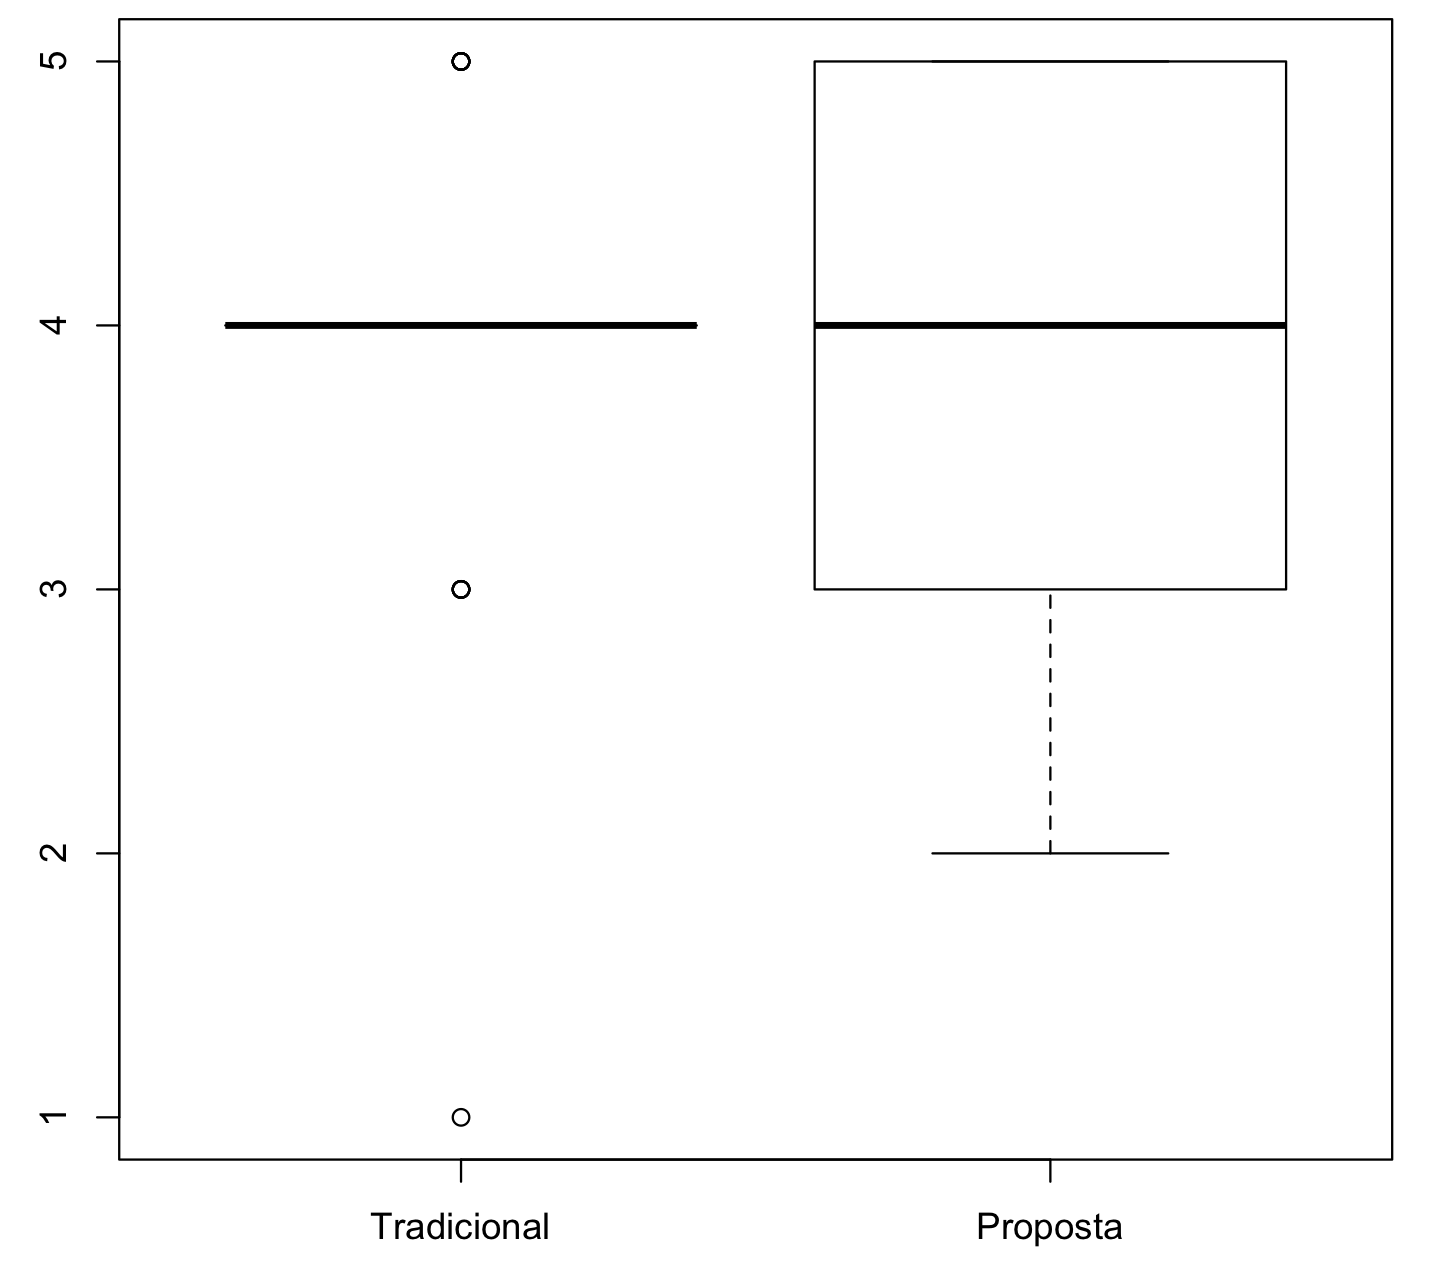
\includegraphics[scale=0.4]{./Figuras/questao4-boxplot.png}
  \end{center}
  \legend{Fonte: O autor.}
\end{figure}

\begin{multicols}{2}

\noindent\textbf{Tradicional}\\
Min.   :1.000\\
1st Qu.:4.000\\
Median :4.000\\
Mean   :3.931\\
3rd Qu.:4.000\\
Max.   :5.000\\
\columnbreak

\noindent\textbf{Proposta}\\
Min.   :2\\
1st Qu.:3\\
Median :4\\
Mean   :4\\
3rd Qu.:5\\
Max.   :5
\end{multicols}

Wilcoxon rank sum test with continuity correction

\noindent
data:  $data\_4\_tradicional$ and $data\_4\_proposta$\\
W = 378, p-value = 0.8198\\
alternative hypothesis: true location shift is not equal to 0

\textbf{Resultado: Aceita a hipótese nula - Sem diferença significativa}

\newpage
\textbf{Questão 5: O sistema de recomendação explica porque os links são recomendados para mim.}

\begin{figure}[htb]
  \caption{\label{fig:questao5-boxplot}Boxplot da questão 5}
  \begin{center}
      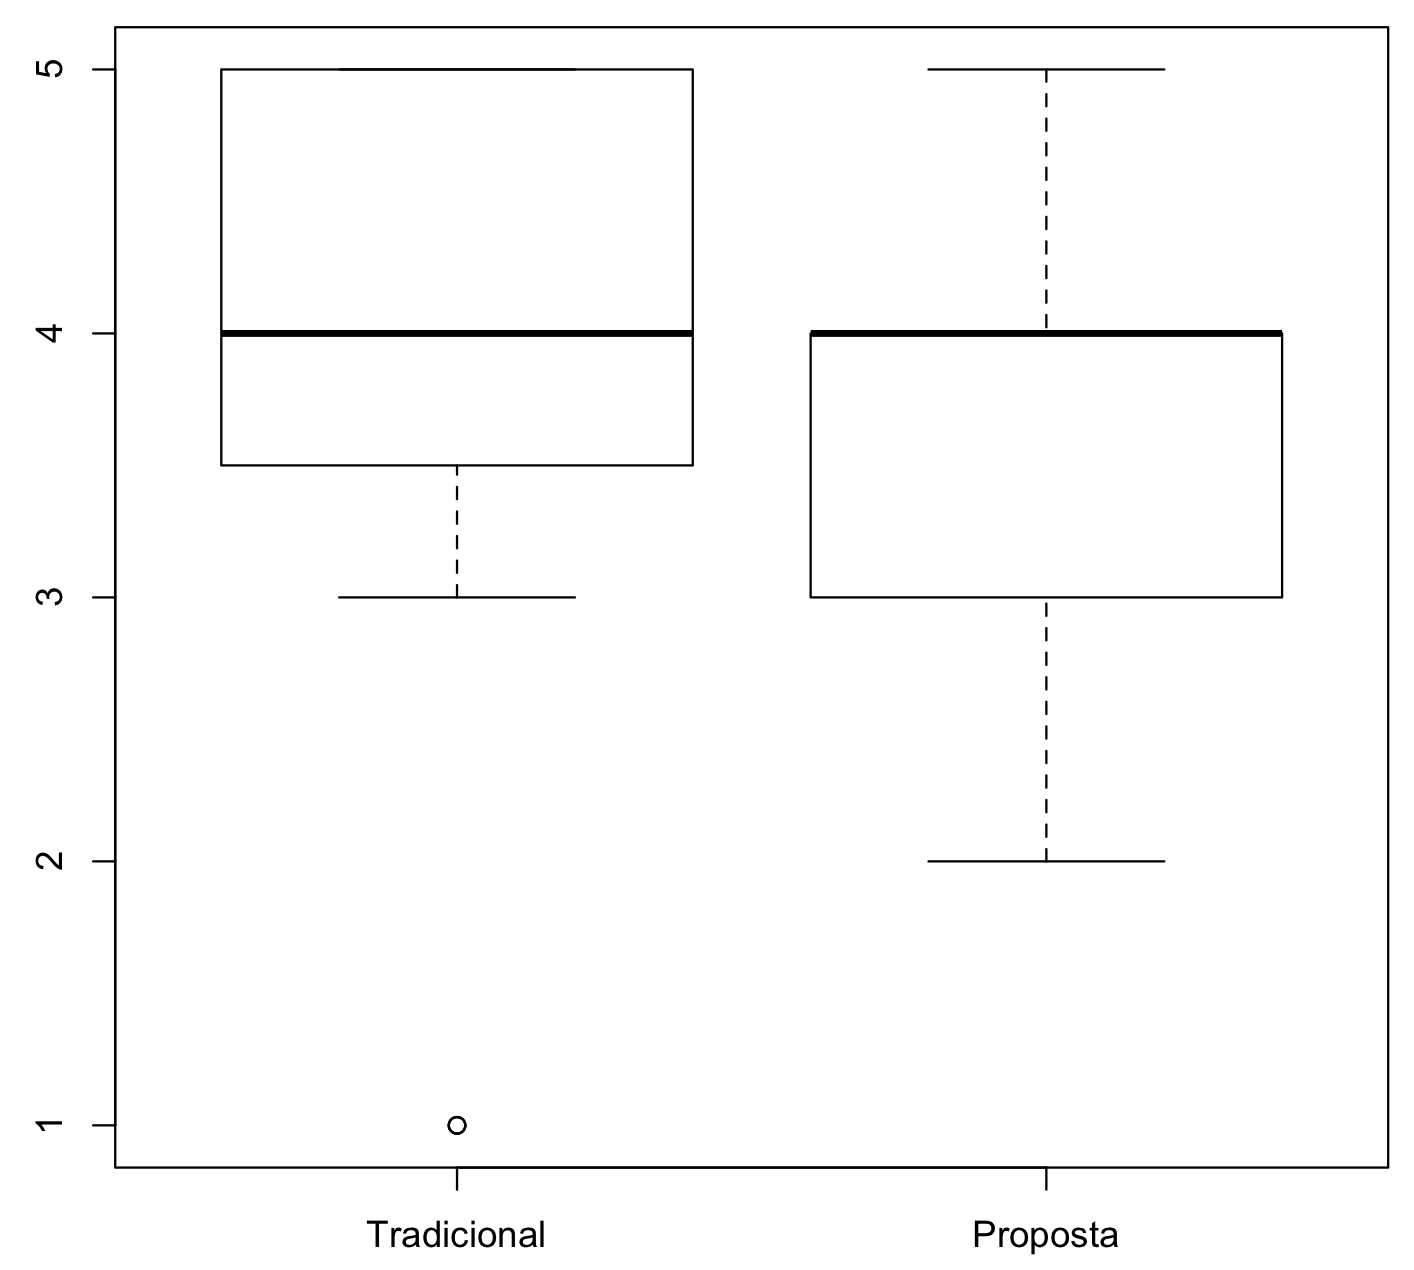
\includegraphics[scale=0.4]{./Figuras/questao5-boxplot.png}
  \end{center}
  \legend{Fonte: O autor.}
\end{figure}

\begin{multicols}{2}

\noindent\textbf{Tradicional}\\
Min.   :1.000\\
1st Qu.:3.500\\
Median :4.000\\
Mean   :3.889\\
3rd Qu.:5.000\\
Max.   :5.000\\
\columnbreak

\noindent\textbf{Proposta}\\
Min.   :2.00\\
1st Qu.:3.00\\
Median :4.00\\
Mean   :3.72\\
3rd Qu.:4.00\\
Max.   :5.00
\end{multicols}

Wilcoxon rank sum test with continuity correction

\noindent
data:  $data\_5\_tradicional$ and $data\_5\_proposta$\\
W = 396, p-value = 0.2665\\
alternative hypothesis: true location shift is not equal to 0

\textbf{Resultado: Aceita a hipótese nula - Sem diferença significativa}

\newpage
\textbf{Questão 6: A informação apresentada na interface para os itens recomendados é suficiente para mim.}

\begin{figure}[htb]
  \caption{\label{fig:questao6-boxplot}Boxplot da questão 6}
  \begin{center}
      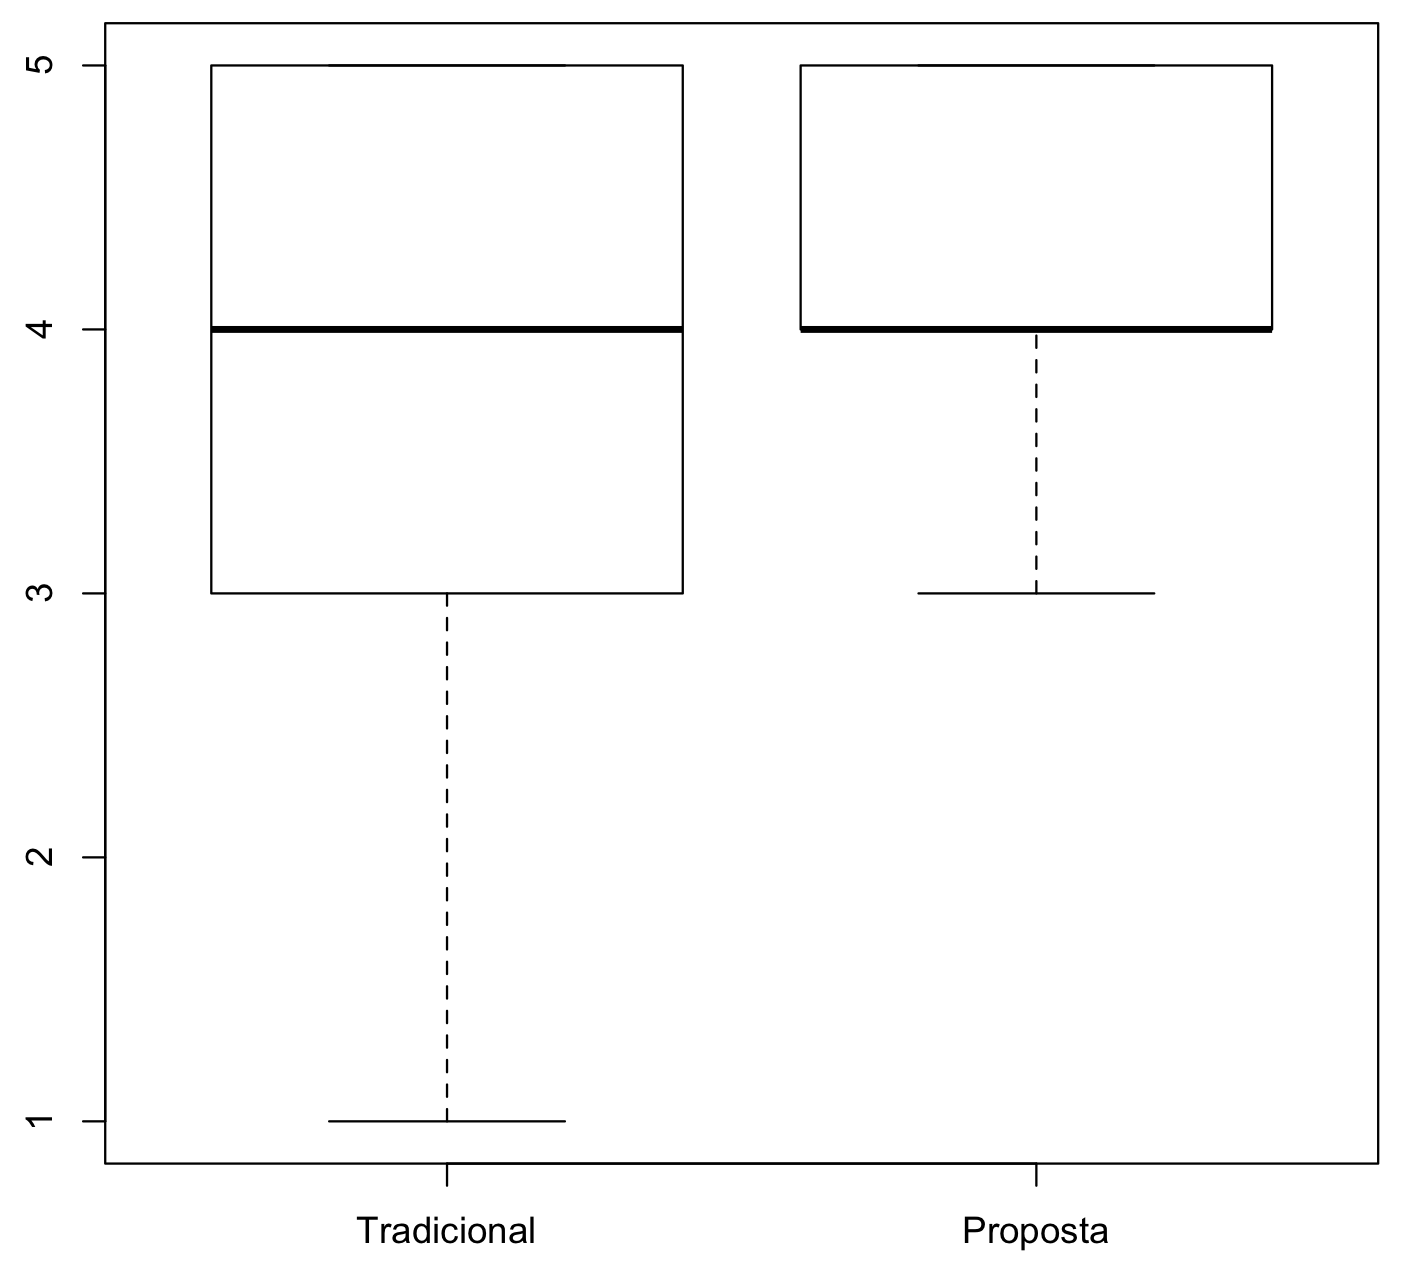
\includegraphics[scale=0.4]{./Figuras/questao6-boxplot.png}
  \end{center}
  \legend{Fonte: O autor.}
\end{figure}

\begin{multicols}{2}

\noindent\textbf{Tradicional}\\
Min.   :1.000\\
1st Qu.:3.000\\
Median :4.000\\
Mean   :3.655\\
3rd Qu.:5.000\\
Max.   :5.000\\
\columnbreak

\noindent\textbf{Proposta}\\
Min.   :3.000\\
1st Qu.:4.000\\
Median :4.000\\
Mean   :4.192\\
3rd Qu.:5.000\\
Max.   :5.000
\end{multicols}

Wilcoxon rank sum test with continuity correction

\noindent
data:  $data\_6\_tradicional$ and $data\_6\_proposta$\\
W = 301.5, p-value = 0.1799\\
alternative hypothesis: true location shift is not equal to 0

\textbf{Resultado: Aceita a hipótese nula - Sem diferença significativa}

\newpage
\textbf{Questão 7: O layout do sistema de recomendação é atrativo e adequado.}

\begin{figure}[htb]
  \caption{\label{fig:questao7-boxplot}Boxplot da questão 7}
  \begin{center}
      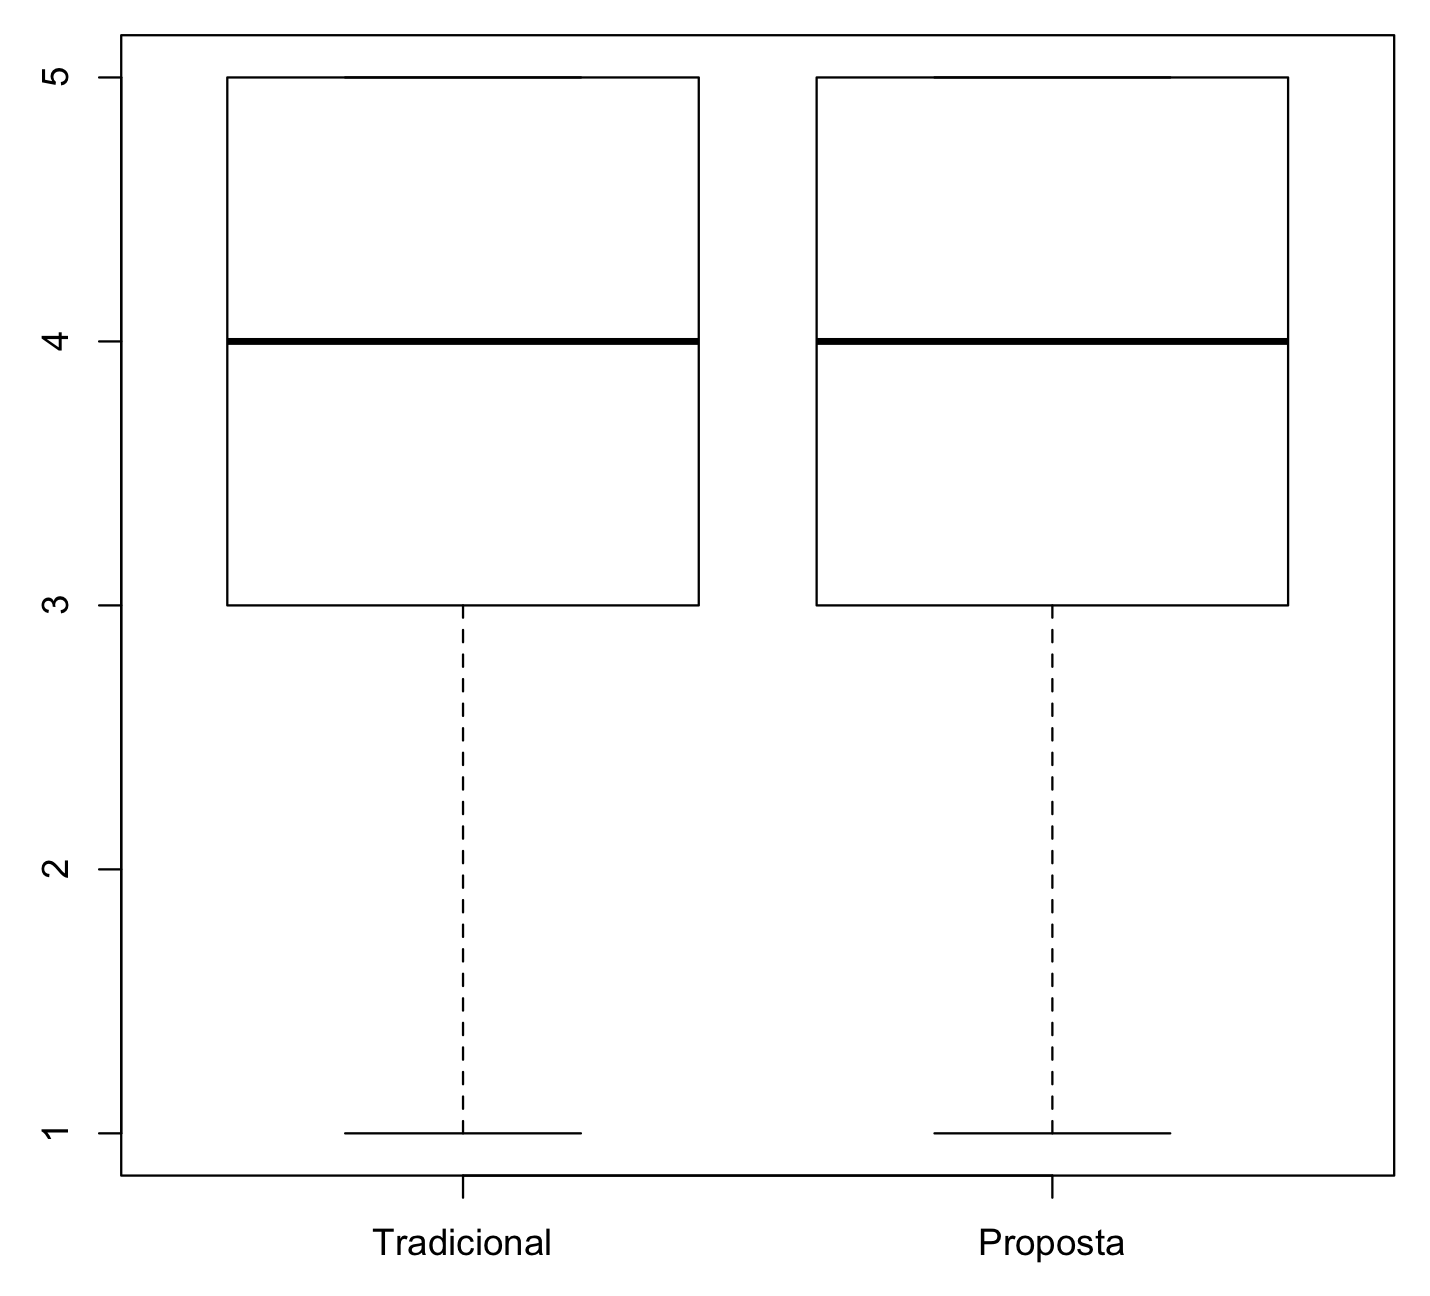
\includegraphics[scale=0.4]{./Figuras/questao7-boxplot.png}
  \end{center}
  \legend{Fonte: O autor.}
\end{figure}

\begin{multicols}{2}

\noindent\textbf{Tradicional}\\
Min.   :1.000\\
1st Qu.:3.000\\
Median :4.000\\
Mean   :3.676\\
3rd Qu.:4.750\\
Max.   :5.000\\
\columnbreak

\noindent\textbf{Proposta}\\
Min.   :1.0\\
1st Qu.:3.0\\
Median :4.0\\
Mean   :3.8\\
3rd Qu.:5.0\\
Max.   :5.0
\end{multicols}

Wilcoxon rank sum test with continuity correction

\noindent
data:  $data\_7\_tradicional$ and $data\_7\_proposta$\\
W = 413, p-value = 0.8536\\
alternative hypothesis: true location shift is not equal to 0

\textbf{Resultado: Aceita a hipótese nula - Sem diferença significativa}

\newpage
\textbf{Questão 8: Eu encontrei facilmente o local onde os itens são recomendados.}

\begin{figure}[htb]
  \caption{\label{fig:questao8-boxplot}Boxplot da questão 8}
  \begin{center}
      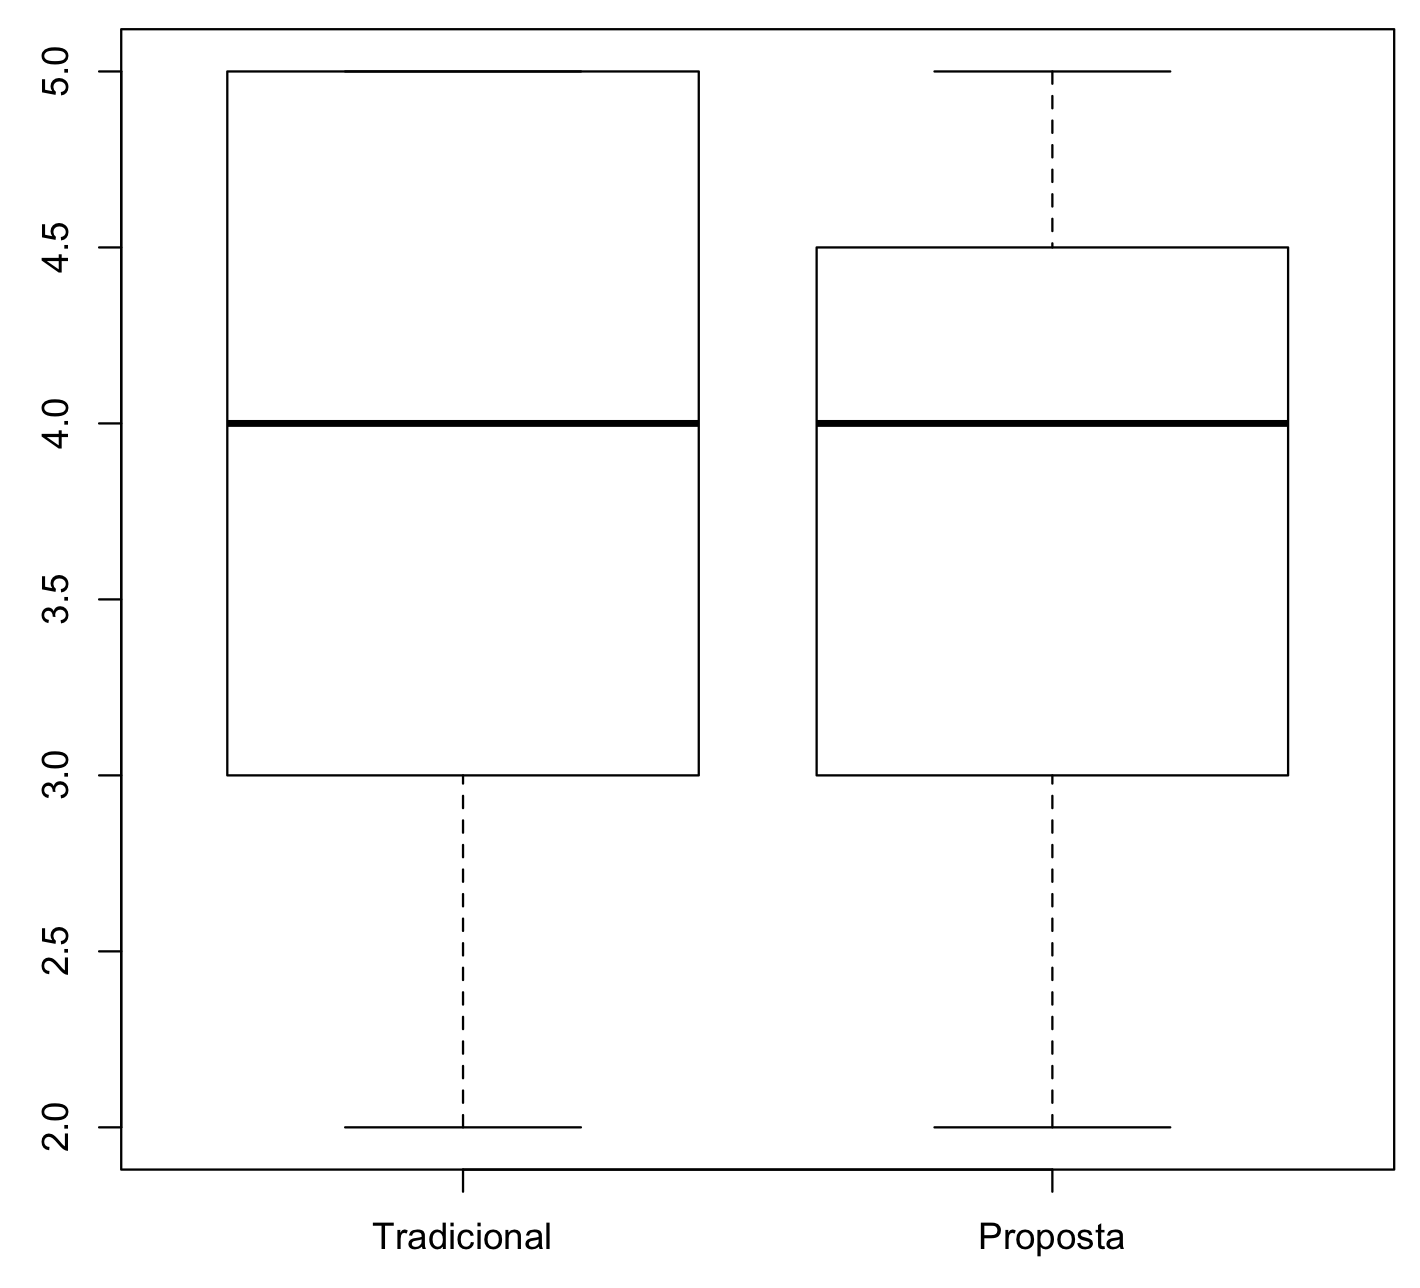
\includegraphics[scale=0.4]{./Figuras/questao8-boxplot.png}
  \end{center}
  \legend{Fonte: O autor.}
\end{figure}

\begin{multicols}{2}

\noindent\textbf{Tradicional}\\
Min.   :2.0\\
1st Qu.:3.0\\
Median :4.0\\
Mean   :3.8\\
3rd Qu.:5.0\\
Max.   :5.0\\
\columnbreak

\noindent\textbf{Proposta}\\
Min.   :2.00\\
1st Qu.:3.00\\
Median :4.00\\
Mean   :3.75\\
3rd Qu.:4.25\\
Max.   :5.00
\end{multicols}

Wilcoxon rank sum test with continuity correction

\noindent
data:  $data\_8\_tradicional$ and $data\_8\_proposta$\\
W = 381, p-value = 0.7093\\
alternative hypothesis: true location shift is not equal to 0

\textbf{Resultado: Aceita a hipótese nula - Sem diferença significativa}

\newpage
\textbf{Questão 9: Eu percebi que o sistema de recomendação aprendia sobre minhas necessidades/preferências conforme eu avançava na disciplina.}

\begin{figure}[htb]
  \caption{\label{fig:questao9-boxplot}Boxplot da questão 9}
  \begin{center}
      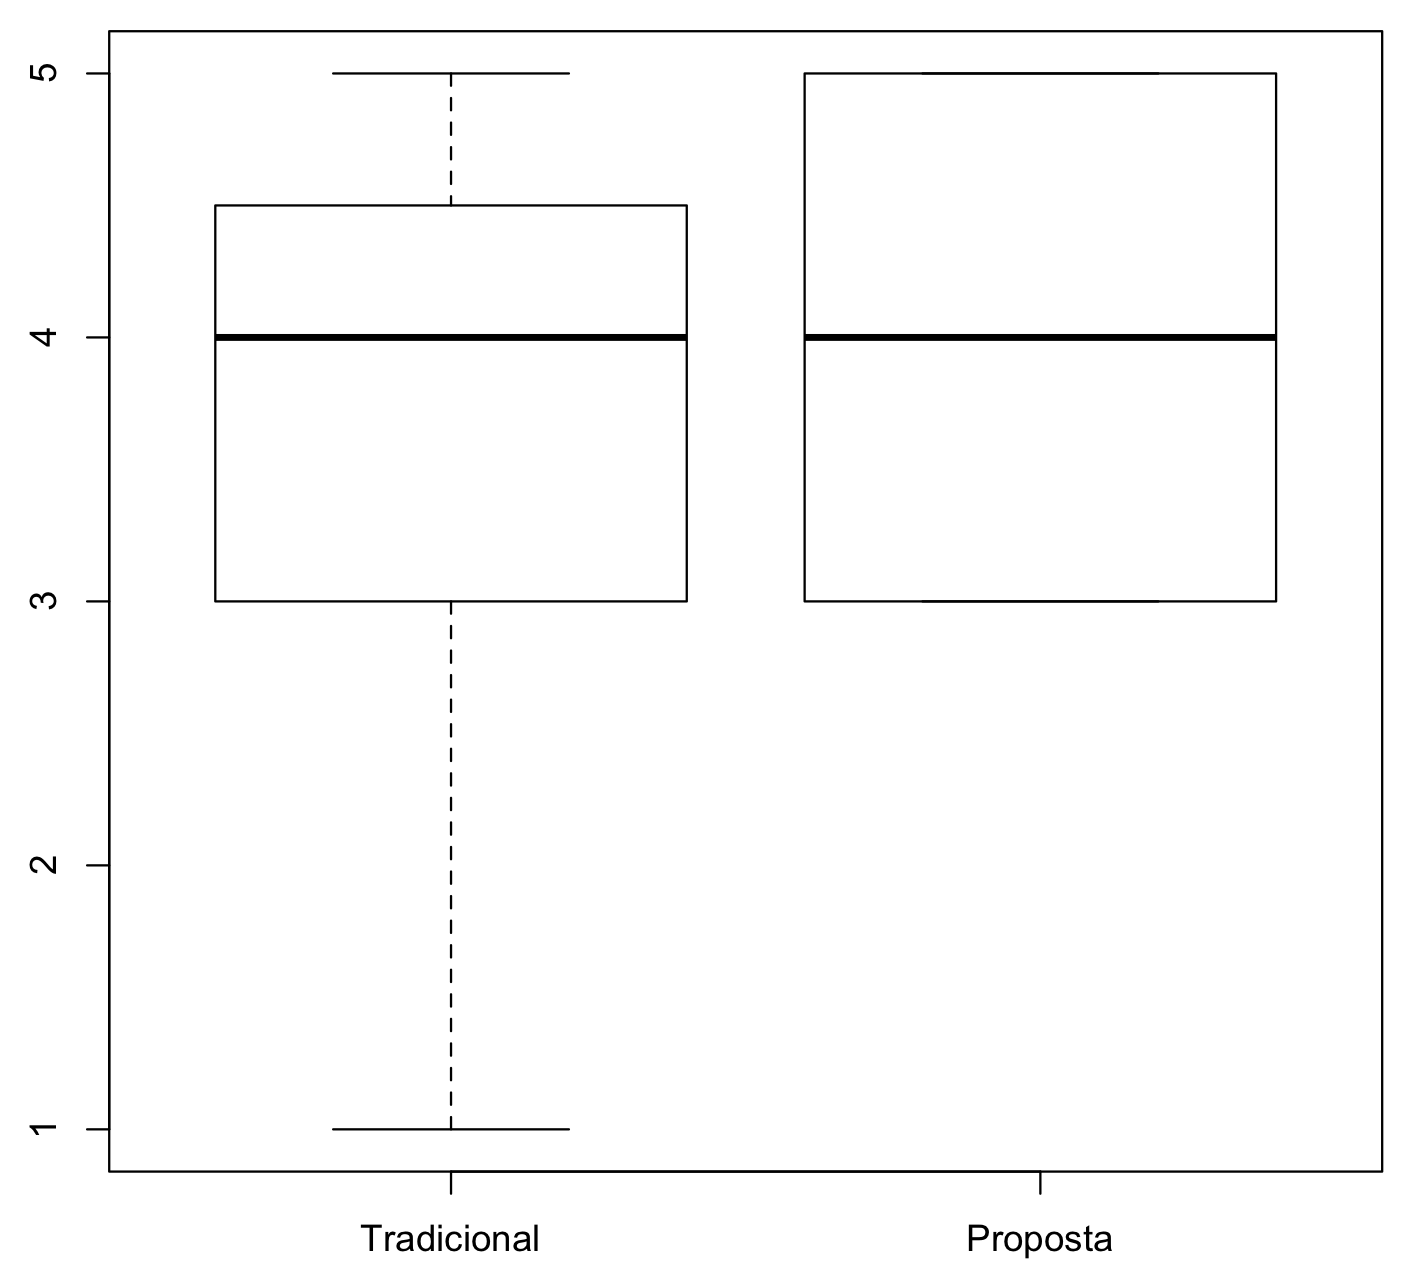
\includegraphics[scale=0.4]{./Figuras/questao9-boxplot.png}
  \end{center}
  \legend{Fonte: O autor.}
\end{figure}

\begin{multicols}{2}

\noindent\textbf{Tradicional}\\
Min.   :1.000\\
1st Qu.:3.000\\
Median :4.000\\
Mean   :3.643\\
3rd Qu.:4.250\\
Max.   :5.000\\
\columnbreak

\noindent\textbf{Proposta}\\
Min.   :3.000\\
1st Qu.:3.000\\
Median :4.000\\
Mean   :3.875\\
3rd Qu.:5.000\\
Max.   :5.000
\end{multicols}

Wilcoxon rank sum test with continuity correction

\noindent
data:  $data\_9\_tradicional$ and $data\_9\_proposta$\\
W = 313.5, p-value = 0.6722\\
alternative hypothesis: true location shift is not equal to 0

\textbf{Resultado: Aceita a hipótese nula - Sem diferença significativa}

\newpage
\textbf{Questão 10: É facil encontrar um item para estudar com a ajuda do sistema de recomendação.}

\begin{figure}[htb]
  \caption{\label{fig:questao10-boxplot}Boxplot da questão 10}
  \begin{center}
      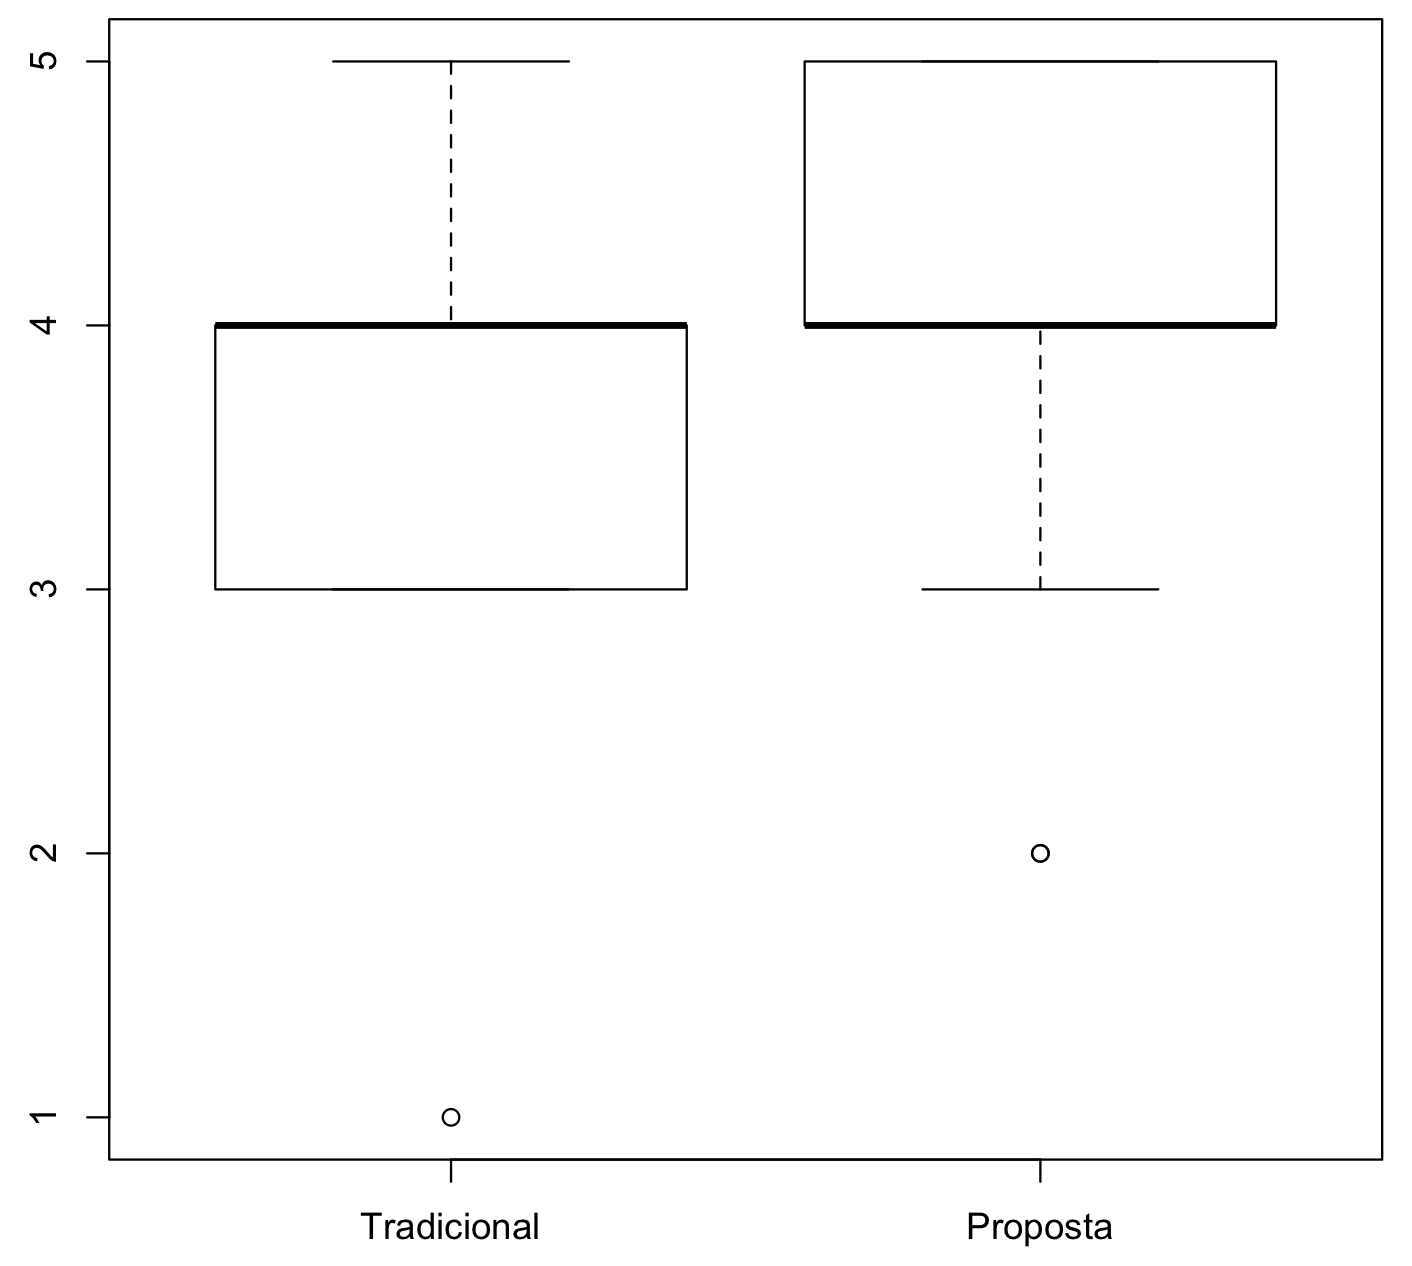
\includegraphics[scale=0.4]{./Figuras/questao10-boxplot.png}
  \end{center}
  \legend{Fonte: O autor.}
\end{figure}

\begin{multicols}{2}

\noindent\textbf{Tradicional}\\
Min.   :1.00\\
1st Qu.:3.00\\
Median :4.00\\
Mean   :3.69\\
3rd Qu.:4.00\\
Max.   :5.00\\
\columnbreak

\noindent\textbf{Proposta}\\
Min.   :2\\
1st Qu.:4\\
Median :4\\
Mean   :4\\
3rd Qu.:5\\
Max.   :5
\end{multicols}

Wilcoxon rank sum test with continuity correction

\noindent
data:  $data\_10\_tradicional$ and $data\_10\_proposta$\\
W = 296, p-value = 0.1452\\
alternative hypothesis: true location shift is not equal to 0

\textbf{Resultado: Aceita a hipótese nula - Sem diferença significativa}

\newpage
\textbf{Questão 11: Eu me senti apoiado para encontrar itens do meu interesse com a ajuda do sistema de recomendação.}

\begin{figure}[htb]
  \caption{\label{fig:questao11-boxplot}Boxplot da questão 11}
  \begin{center}
      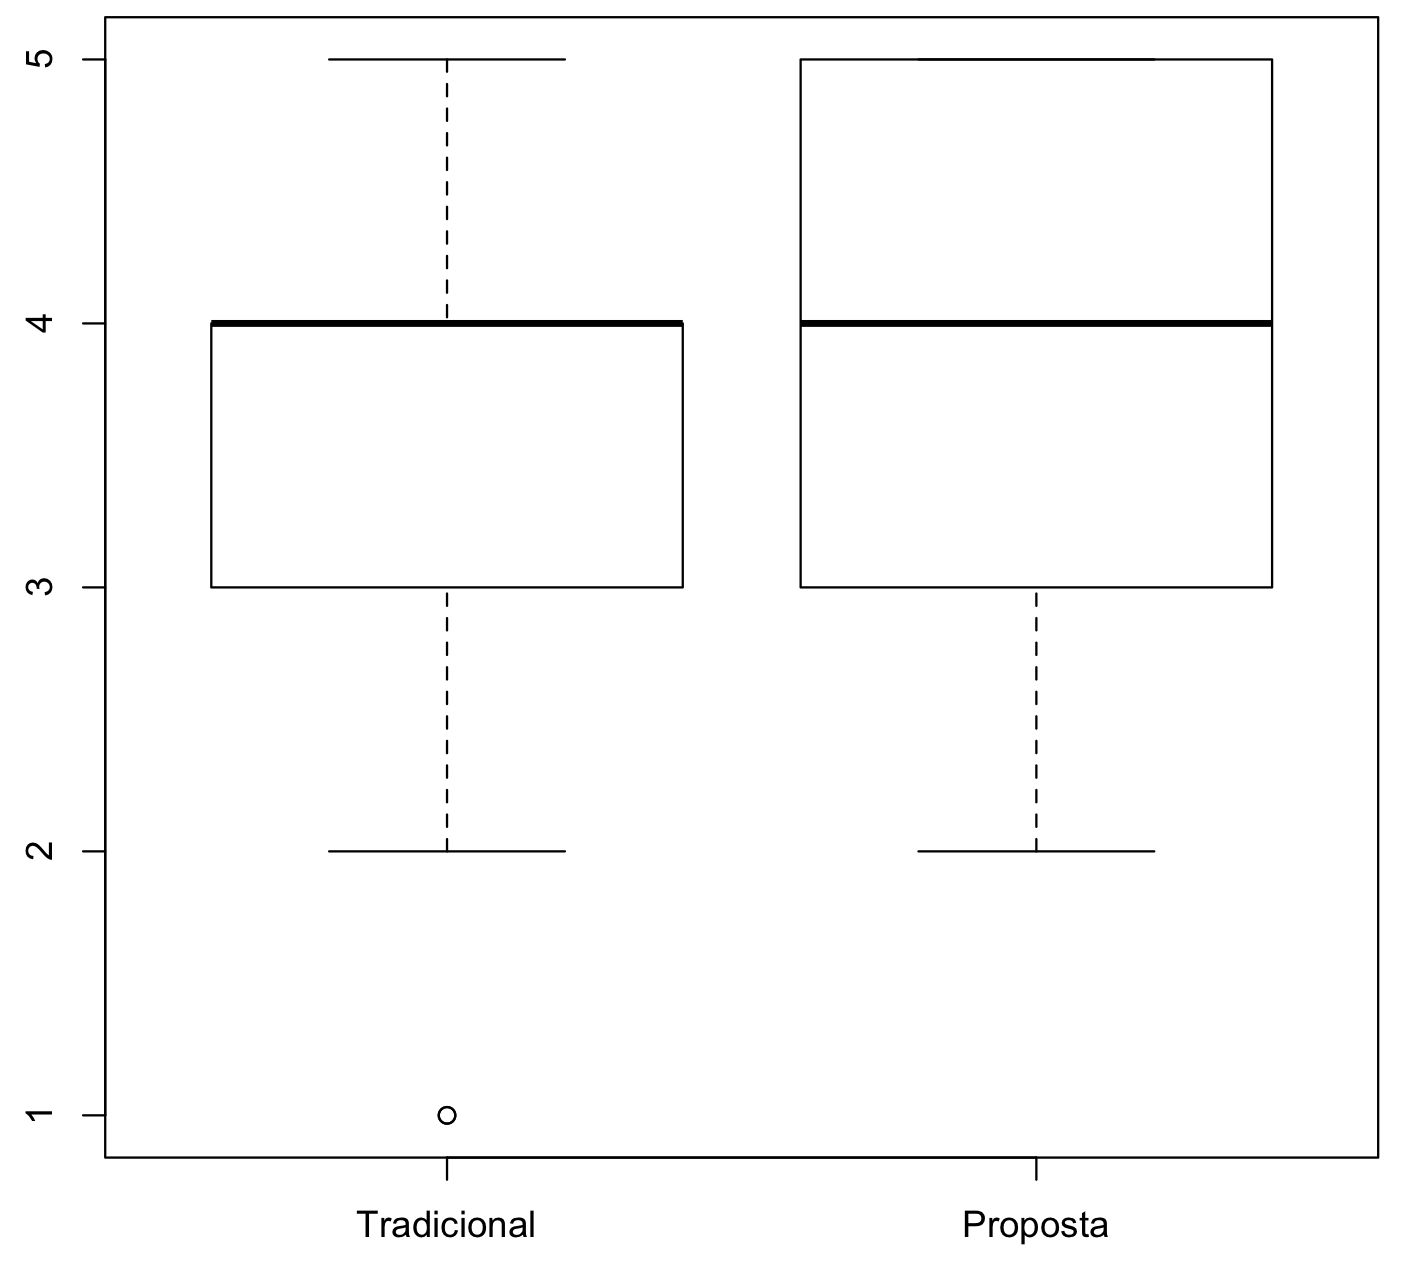
\includegraphics[scale=0.4]{./Figuras/questao11-boxplot.png}
  \end{center}
  \legend{Fonte: O autor.}
\end{figure}

\begin{multicols}{2}

\noindent\textbf{Tradicional}\\
Min.   :1.000\\
1st Qu.:3.000\\
Median :4.000\\
Mean   :3.607\\
3rd Qu.:4.000\\
Max.   :5.000\\
\columnbreak

\noindent\textbf{Proposta}\\
Min.   :2\\
1st Qu.:3\\
Median :4\\
Mean   :4\\
3rd Qu.:5\\
Max.   :5
\end{multicols}

Wilcoxon rank sum test with continuity correction

\noindent
data:  $data\_11\_tradicional$ and $data\_11\_proposta$\\
W = 286, p-value = 0.2309\\
alternative hypothesis: true location shift is not equal to 0

\textbf{Resultado: Aceita a hipótese nula - Sem diferença significativa}

\newpage
\textbf{Questão 12: Eu entendi porque os itens foram recomendados para mim.}

\begin{figure}[htb]
  \caption{\label{fig:questao12-boxplot}Boxplot da questão 12}
  \begin{center}
      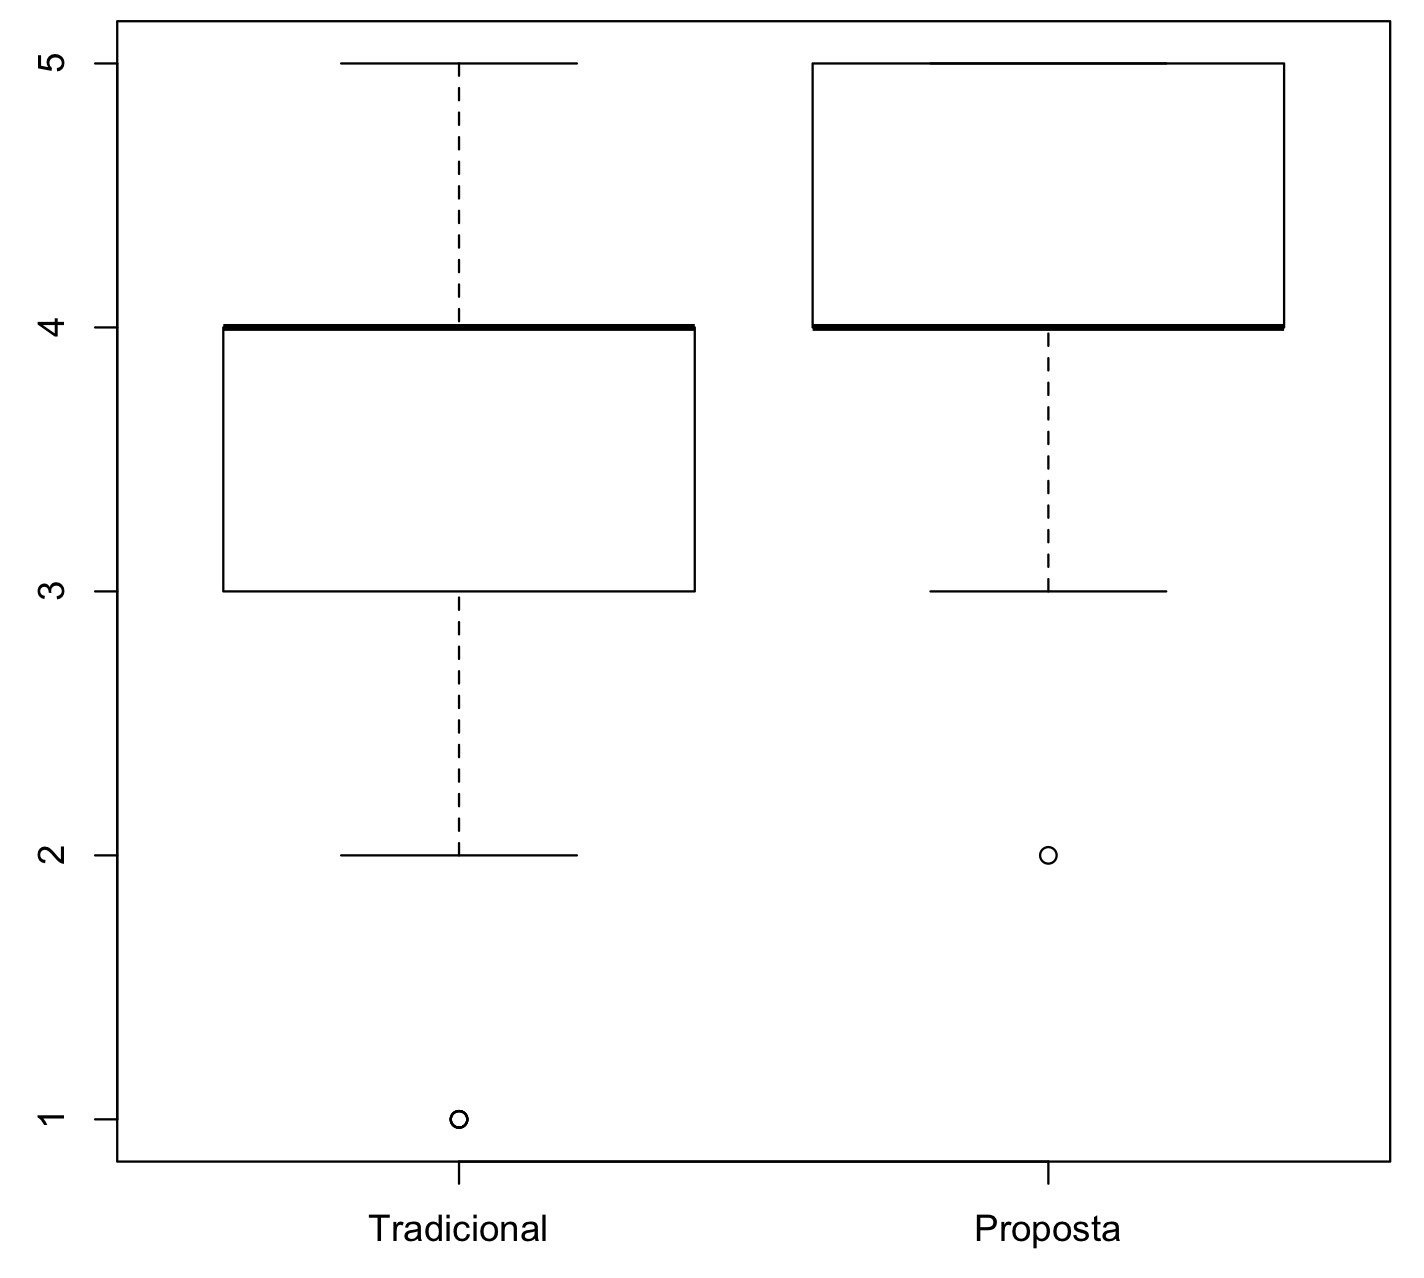
\includegraphics[scale=0.4]{./Figuras/questao12-boxplot.png}
  \end{center}
  \legend{Fonte: O autor.}
\end{figure}

\begin{multicols}{2}

\noindent\textbf{Tradicional}\\
Min.   :1.0\\
1st Qu.:3.0\\
Median :4.0\\
Mean   :3.4\\
3rd Qu.:4.0\\
Max.   :5.0\\
\columnbreak

\noindent\textbf{Proposta}\\
Min.   :2.00\\
1st Qu.:4.00\\
Median :4.00\\
Mean   :4.12\\
3rd Qu.:5.00\\
Max.   :5.00
\end{multicols}

Wilcoxon rank sum test with continuity correction

\noindent
data:  $data\_12\_tradicional$ and $data\_12\_proposta$\\
W = 240, p-value = 0.01513\\
alternative hypothesis: true location shift is not equal to 0

\textbf{Resultado: Aceita a hipótese alternativa - Com diferença significativa}

\newpage
\textbf{Questão 13: No geral, estou satisfeito com o sistema de recomendação.}

\begin{figure}[htb]
  \caption{\label{fig:questao13-boxplot}Boxplot da questão 13}
  \begin{center}
      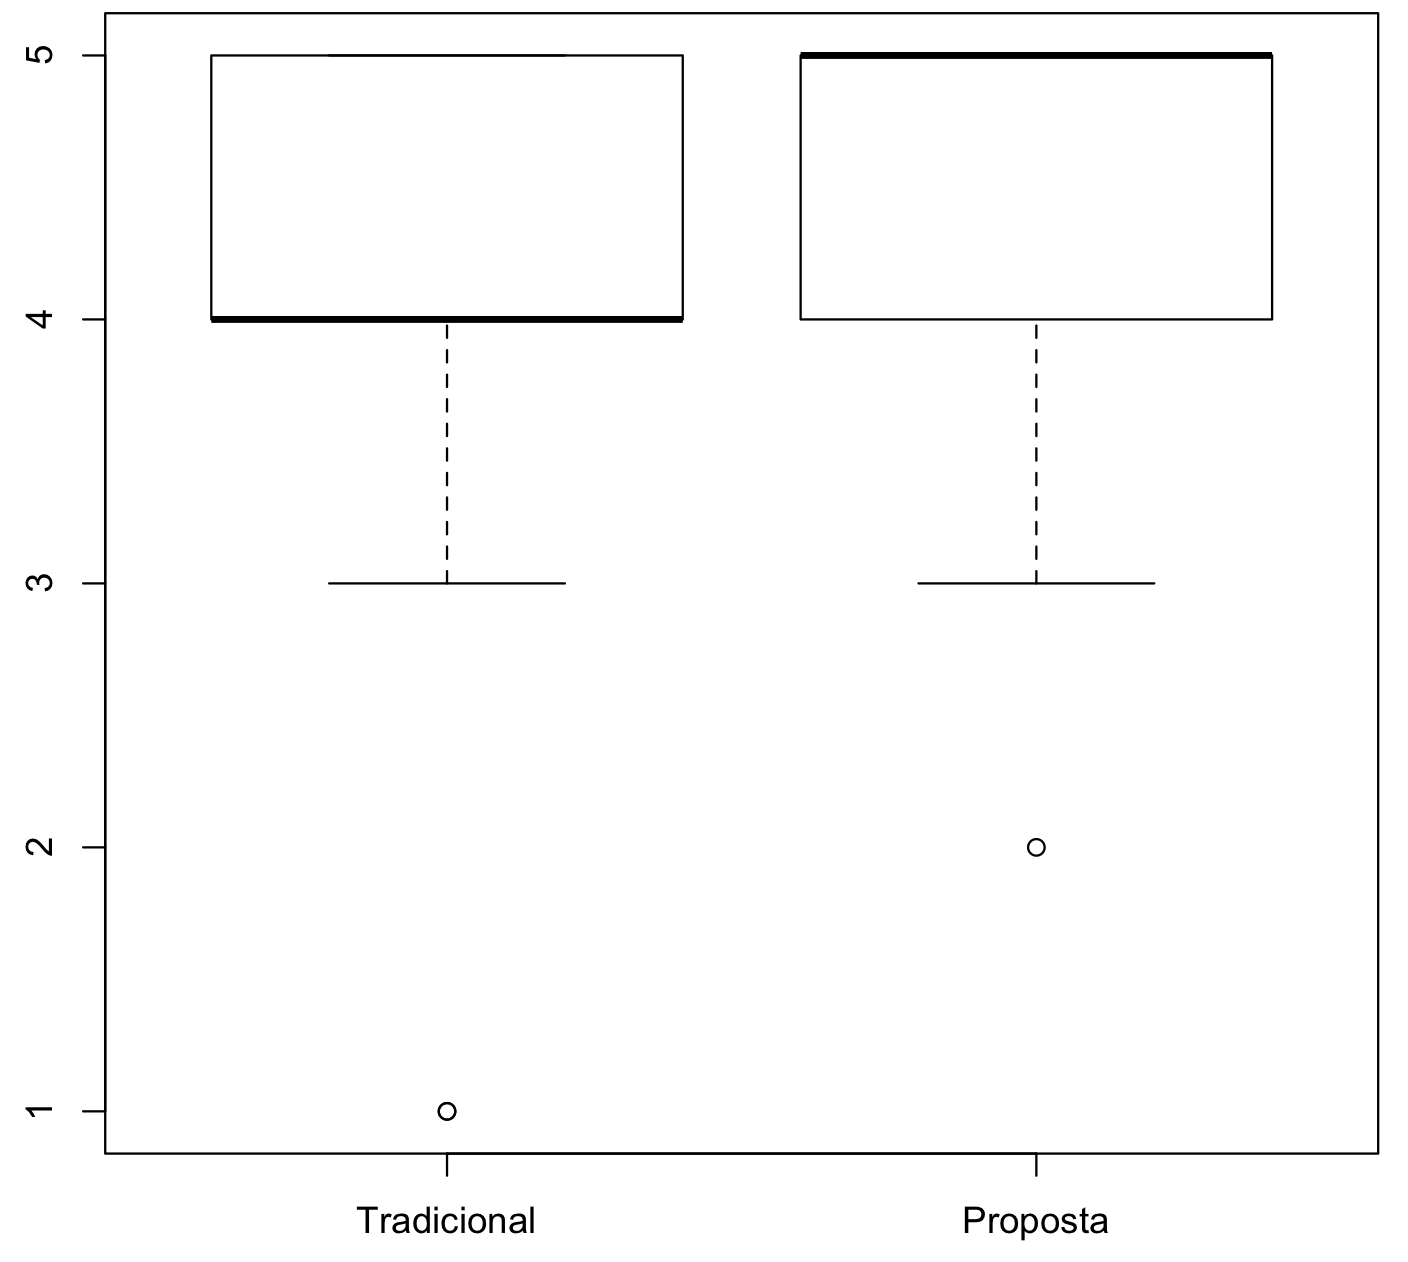
\includegraphics[scale=0.4]{./Figuras/questao13-boxplot.png}
  \end{center}
  \legend{Fonte: O autor.}
\end{figure}

\begin{multicols}{2}

\noindent\textbf{Tradicional}\\
Min.   :1\\
1st Qu.:4\\
Median :4\\
Mean   :4\\
3rd Qu.:5\\
Max.   :5\\
\columnbreak

\noindent\textbf{Proposta}\\
Min.   :2.000\\
1st Qu.:4.000\\
Median :5.000\\
Mean   :4.308\\
3rd Qu.:5.000\\
Max.   :5.000
\end{multicols}

Wilcoxon rank sum test with continuity correction

\noindent
data:  $data\_13\_tradicional$ and $data\_13\_proposta$\\
W = 356.5, p-value = 0.2388\\
alternative hypothesis: true location shift is not equal to 0
